%%=============================================================================
%% Proof of concept
%%=============================================================================

\chapter{\IfLanguageName{dutch}{Proof of Concept}{Proof of Concept}}%
\label{ch:proofofconcept}

% TODO: Trek een duidelijke conclusie, in de vorm van een antwoord op de
% onderzoeksvra(a)g(en). Wat was jouw bijdrage aan het onderzoeksdomein en
% hoe biedt dit meerwaarde aan het vakgebied/doelgroep? 
% Reflecteer kritisch over het resultaat. In Engelse teksten wordt deze sectie
% ``Discussion'' genoemd. Had je deze uitkomst verwacht? Zijn er zaken die nog
% niet duidelijk zijn?
% Heeft het onderzoek geleid tot nieuwe vragen die uitnodigen tot verder 
%onderzoek?

\section{\IfLanguageName{dutch}{Ontwikkeling van de mobiele app}{Development mobile app}}%
\label{sec:ontwikkeling mobiele app}

Om de onderzoeksvraag van deze bachelorproef te kunnen beantwoorden werden een Python web server en een  iOS app ontwikkeld als proof of concept. Deze app maakt in de eerste plaats het elektriciteitsverbruik en de stroomproductie van de zonnepanelen inzichtelijk. Daarnaast zal de app via de toepassing van machine learning de elektriciteitsproductie van de volgende dag voorspellen. Deze voorspelling zal dan door de app gebruikt worden om de inschakeling van twee slimme stekkers te programmeren indien er voldoende stroomproductie voorspeld wordt.

\subsection{\IfLanguageName{dutch}{Digitale elektriciteitsmeter uitlezen}{Reading out digital electricitymeter}}%
\label{sec:Digitale elektriciteitsmeter uitlezen}

Een mobiele app die het elektriciteitsverbruik wil bijsturen en beter spreiden zal de gebruiker ervan allereerst inzicht moeten geven in zijn of haar verbruik. Om de verbruiksgegevens te ontsluiten moet de digitale elektriciteitsmeter uitgelezen worden via de P1-poort. Hiervoor zijn verschillende mogelijkheden, van een dongle tot kleine toestellen die via een kabel met de P1-poort kunnen verbonden worden. Voor dit onderzoek is er gekozen voor een Raspberry Pi 5 minicomputer om de digitale meter uit te lezen. Deze singleboardcomputer die gebaseerd is op een ARM processor en de Linuxdistributie Ubuntu als besturingssysteem heeft, biedt meer mogelijkheden dan enkel het uitlezen van data. Omdat het verbruik ervan zeer laag is, kan dit toestel bovendien continu ingeschakeld blijven. Daarnaast heeft de Raspberry Pi wifi-ondersteuning zodat deze kan verbonden worden met het wifi-netwerk van de woning die als testomgeving gebruikt wordt. Dit maakt het mogelijk om een webserver op te zetten en meteen ook de omvormer van de zonnepanelen van de woning via het wifi-netwerk uit te lezen met de Raspberry Pi (zie volgende sectie). In de testwoning bevindt de digitale elektriciteitsmeter zich namelijk in de kelder, terwijl de omvormer van de zonnepanelen zich op zolder bevindt. Een situatie die wel vaker voorkomt en op deze manier kan worden opgelost.

\begin{figure}[h!]
    \centering
    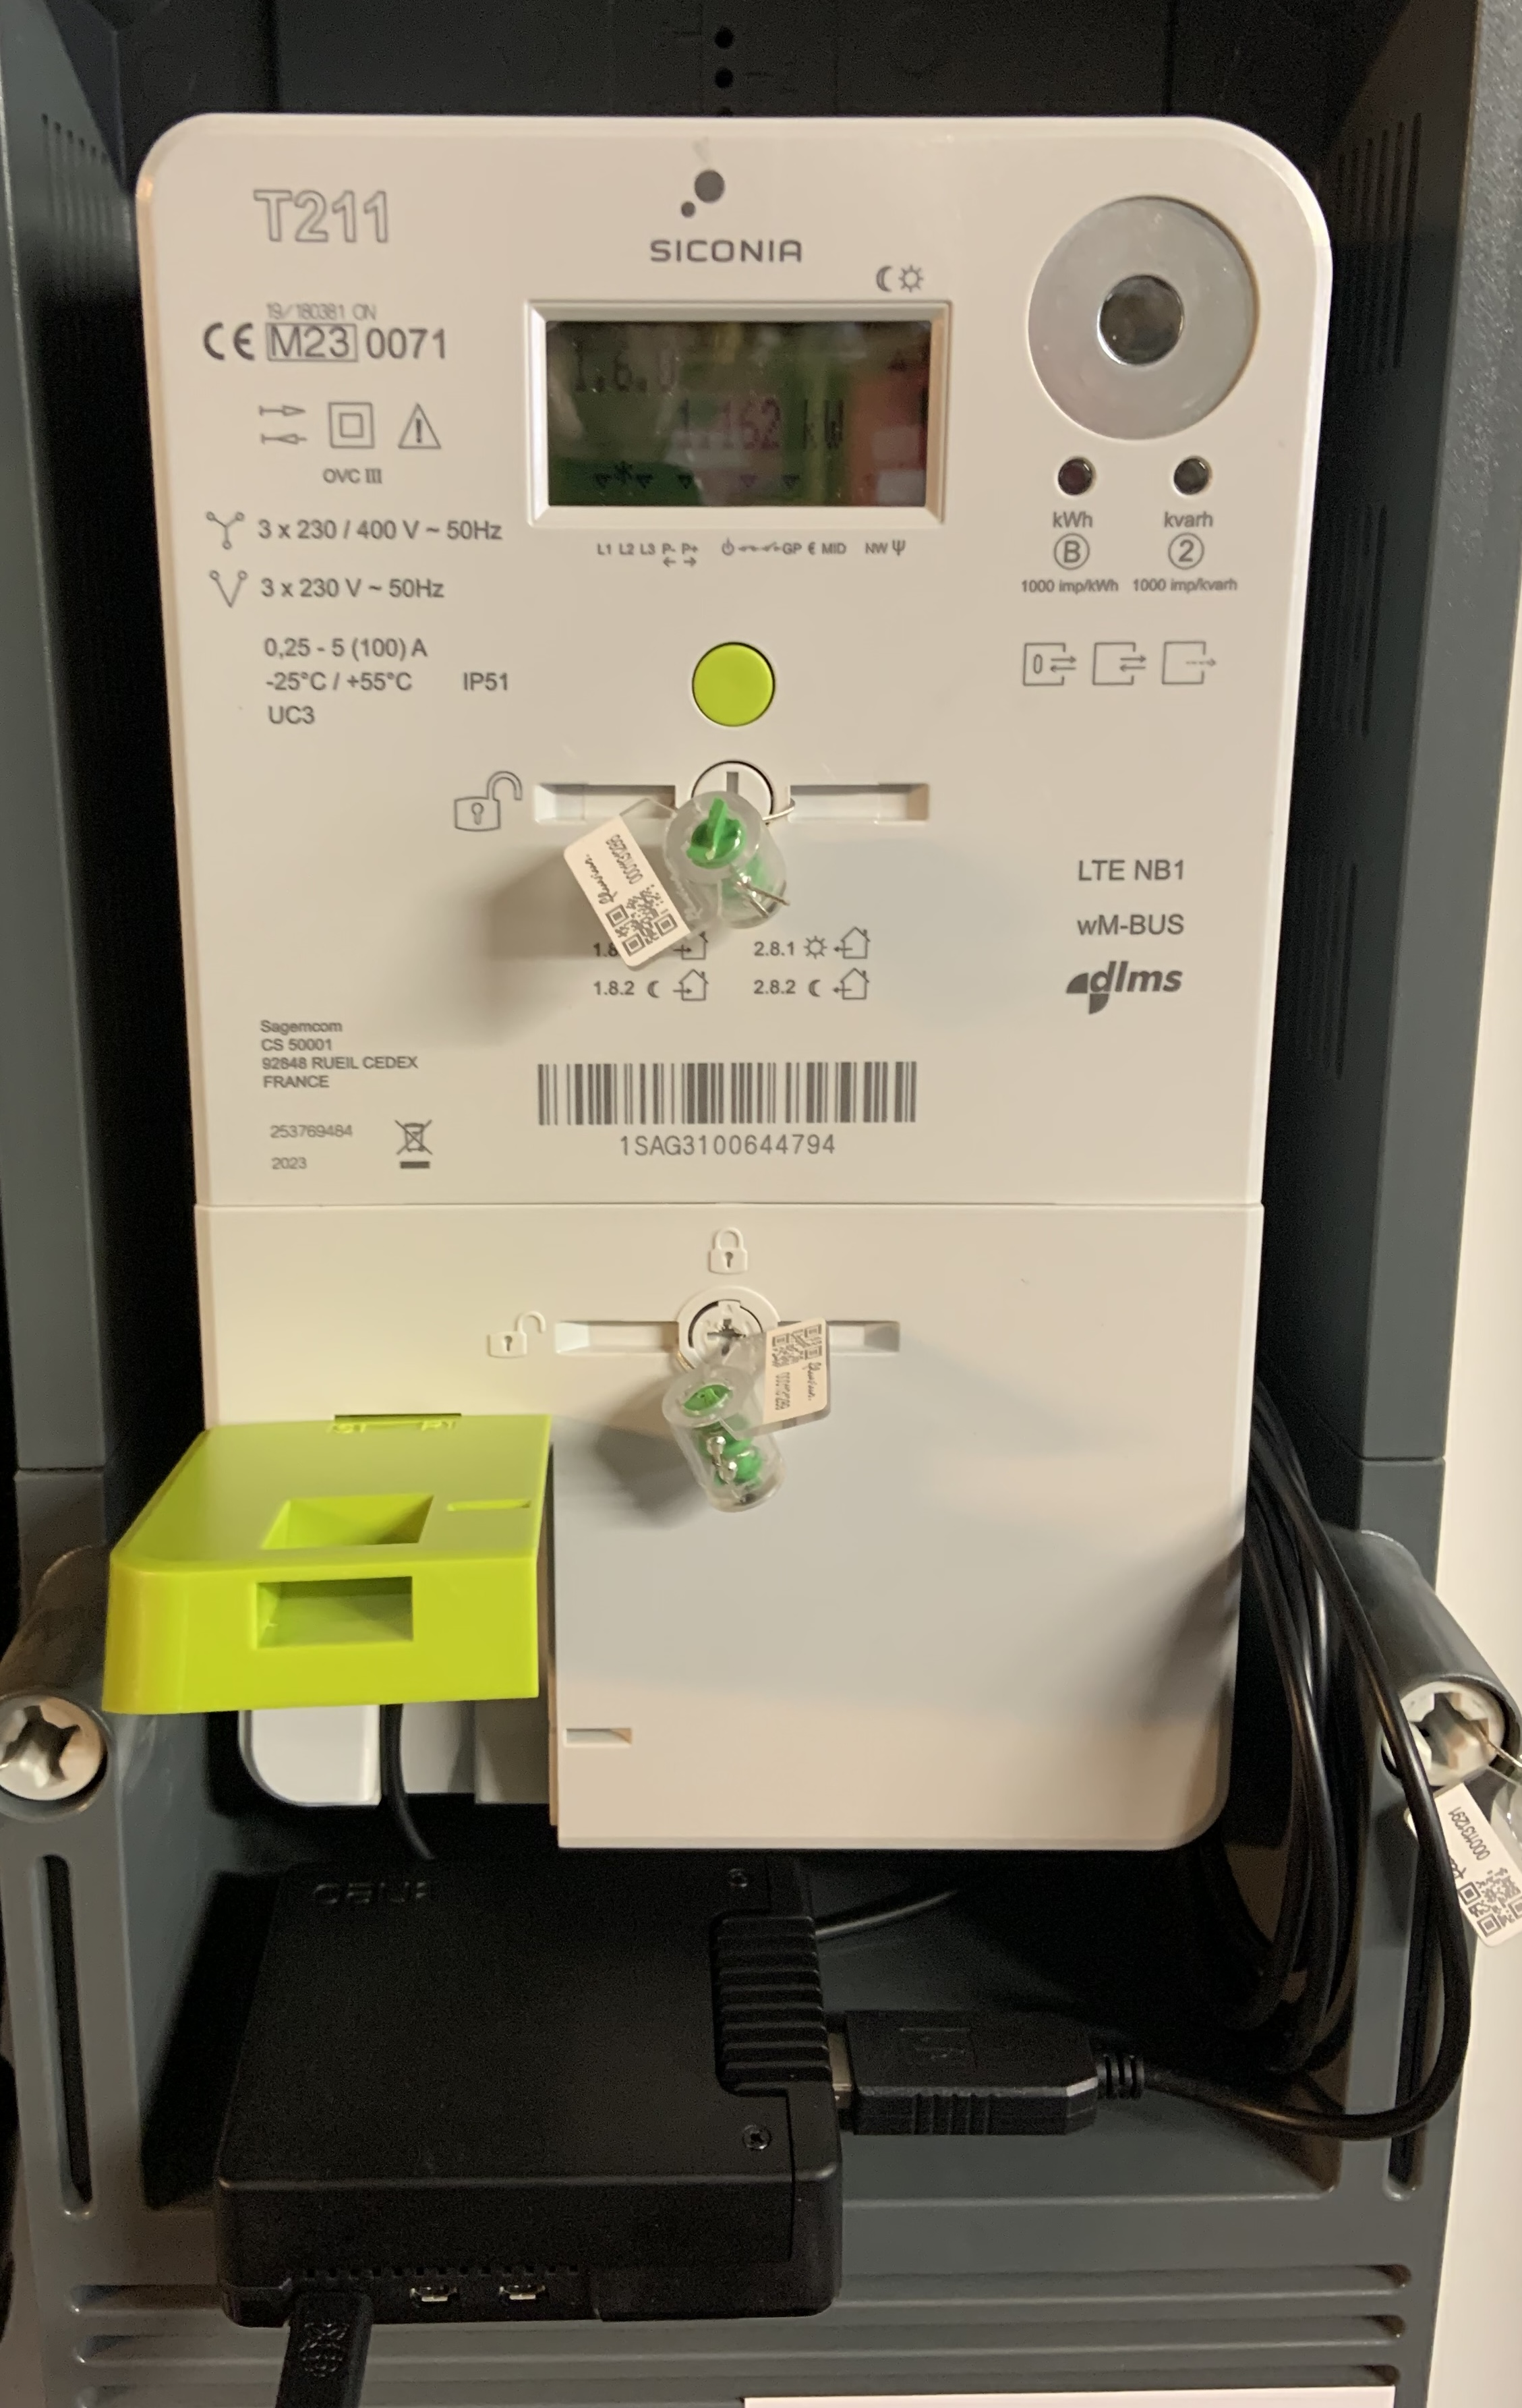
\includegraphics[width=7cm]{TestSetup} \hspace{0.7cm}
    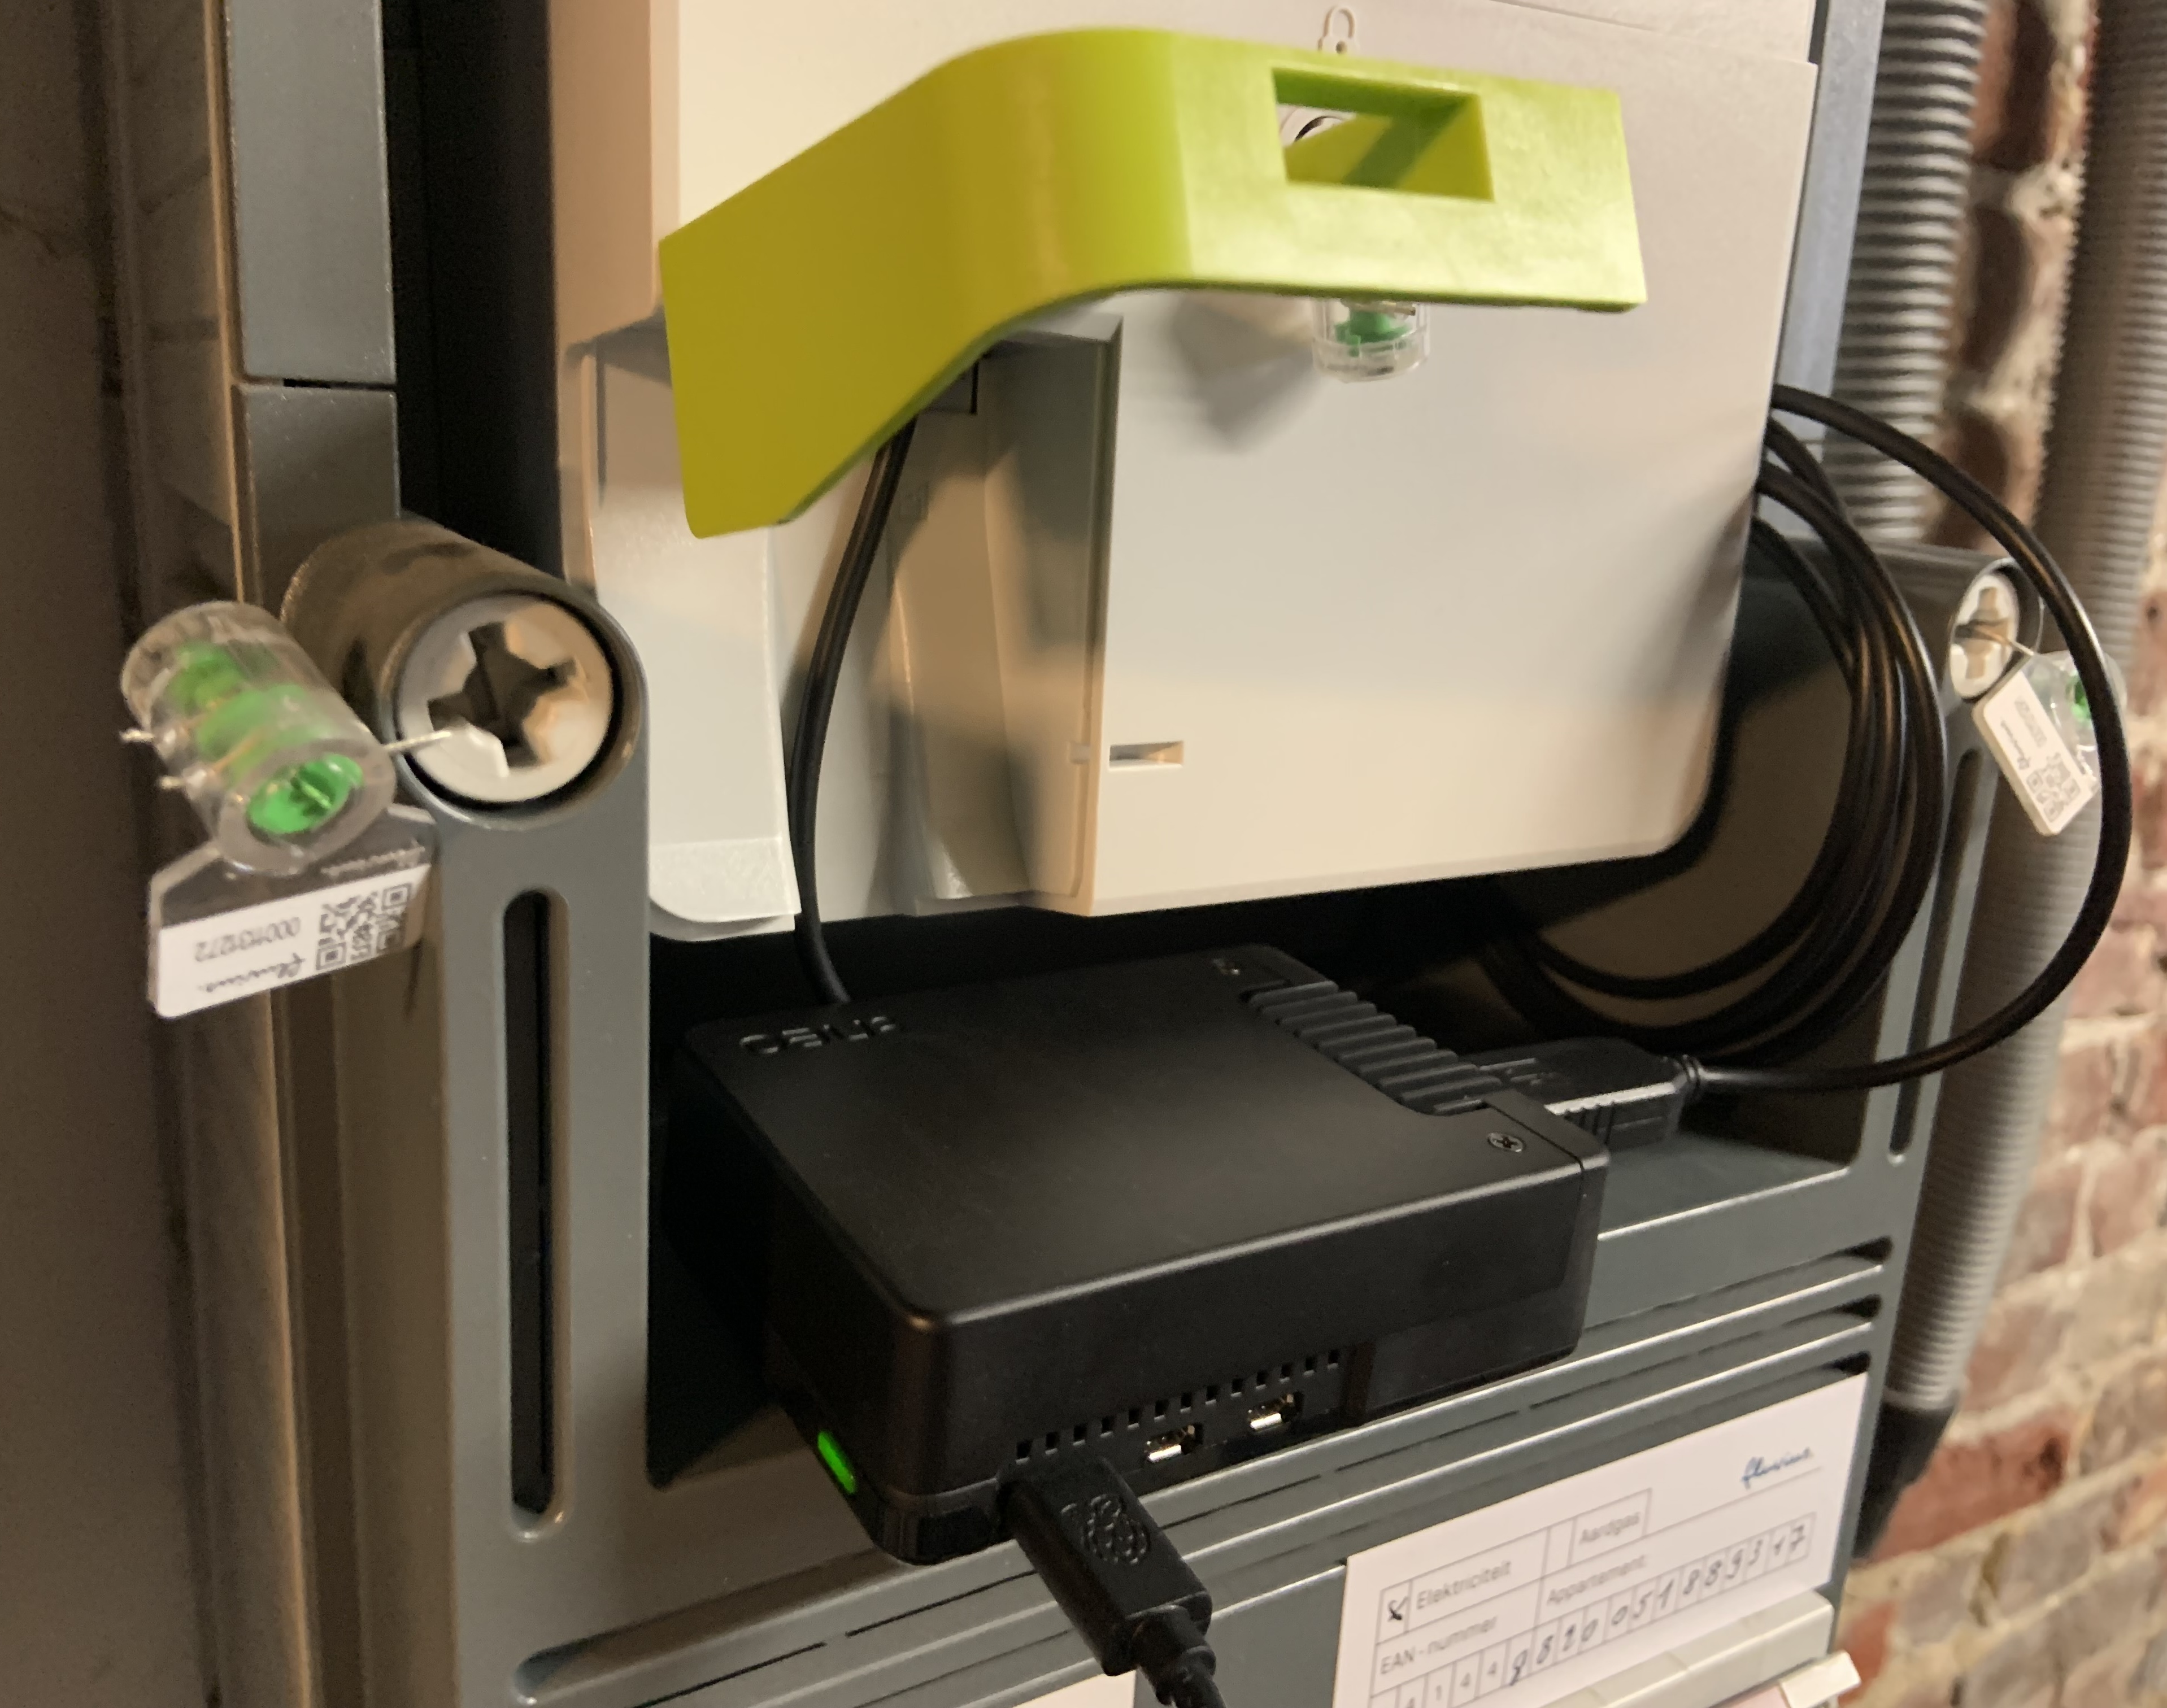
\includegraphics[width=7cm]{RPi5}
    \caption{Testopstelling: Raspberry Pi 5 via een RS422 serieel naar USB kabel aangesloten op een digitale elektriciteitsmeter.}
\end{figure}

\subsubsection{Opslag uitgelezen elektriciteitsdata}

Nadat de Raspberry Pi via de juiste kabel op de P1-poort werd aangesloten, kon de data van de digitale elektriciteitsmeter via een Python script worden uitgelezen. Hiervoor werd een bestaand Python script uitgebreid \autocite{Depuydt2021}. Het bestaande script voorzag enkel in het uitprinten van de uitgelezen data in de console. Om de uitgelezen elektriciteitsdata later via een app te kunnen weergeven moest deze data worden weggeschreven naar een databank. Omdat de data via de P1-poort per seconde uitgelezen wordt, werd geopteerd voor InfluxDB. Deze NoSQL-databank is speciaal ontwikkeld voor time-series en is binnen bepaalde (ruime) grenzen gratis te gebruiken \autocite{Balis2017} en  \autocite{Struckov2019}. Het Python script werd tenslotte opgezet als een achtergrond service via de systeem manager voor Linux 'systemctl/systemd', zodat het voortdurend blijft uitgevoerd worden.

\subsection{\IfLanguageName{dutch}{Omvormer zonnepanelen uitlezen}{Reading out power converter PV system}}%
\label{sec:Omvormer zonnepanelen uitlezen}

Zoals reeds vermeld bevindt de omvormer van de zonnepanelen zich op de zolderverdieping, terwijl de Raspberry Pi zich in de kelder bij de digitale elektriciteitsmeter bevindt. De enige mogelijkheid om een draadloze verbinding te maken tussen beide toestellen is via het lokale wifi-netwerk. De omvormer in casu heeft echter geen ingebouwde wifi-ondersteuning en diende uitgebreid te worden met een aparte wifi-stick. Via deze wifi-stick kon dan vervolgens de data van de omvormer uitgelezen worden. Dit gebeurt opnieuw via een Python script waarin een request wordt gestuurd naar de server van de producent waar de gegevens van de omvormer worden bijgehouden. Omdat de data van de digitale elektriciteitsmeter per seconde wordt uitgelezen, wordt ook de data van de omvormer per seconde opgevraagd. De ontvangen gegevens zijn de temperatuur, de huidige geproduceerde stroom en de totale dagproductie van de zonnepanelen. \\

\begin{figure}[h!]
    \centering
    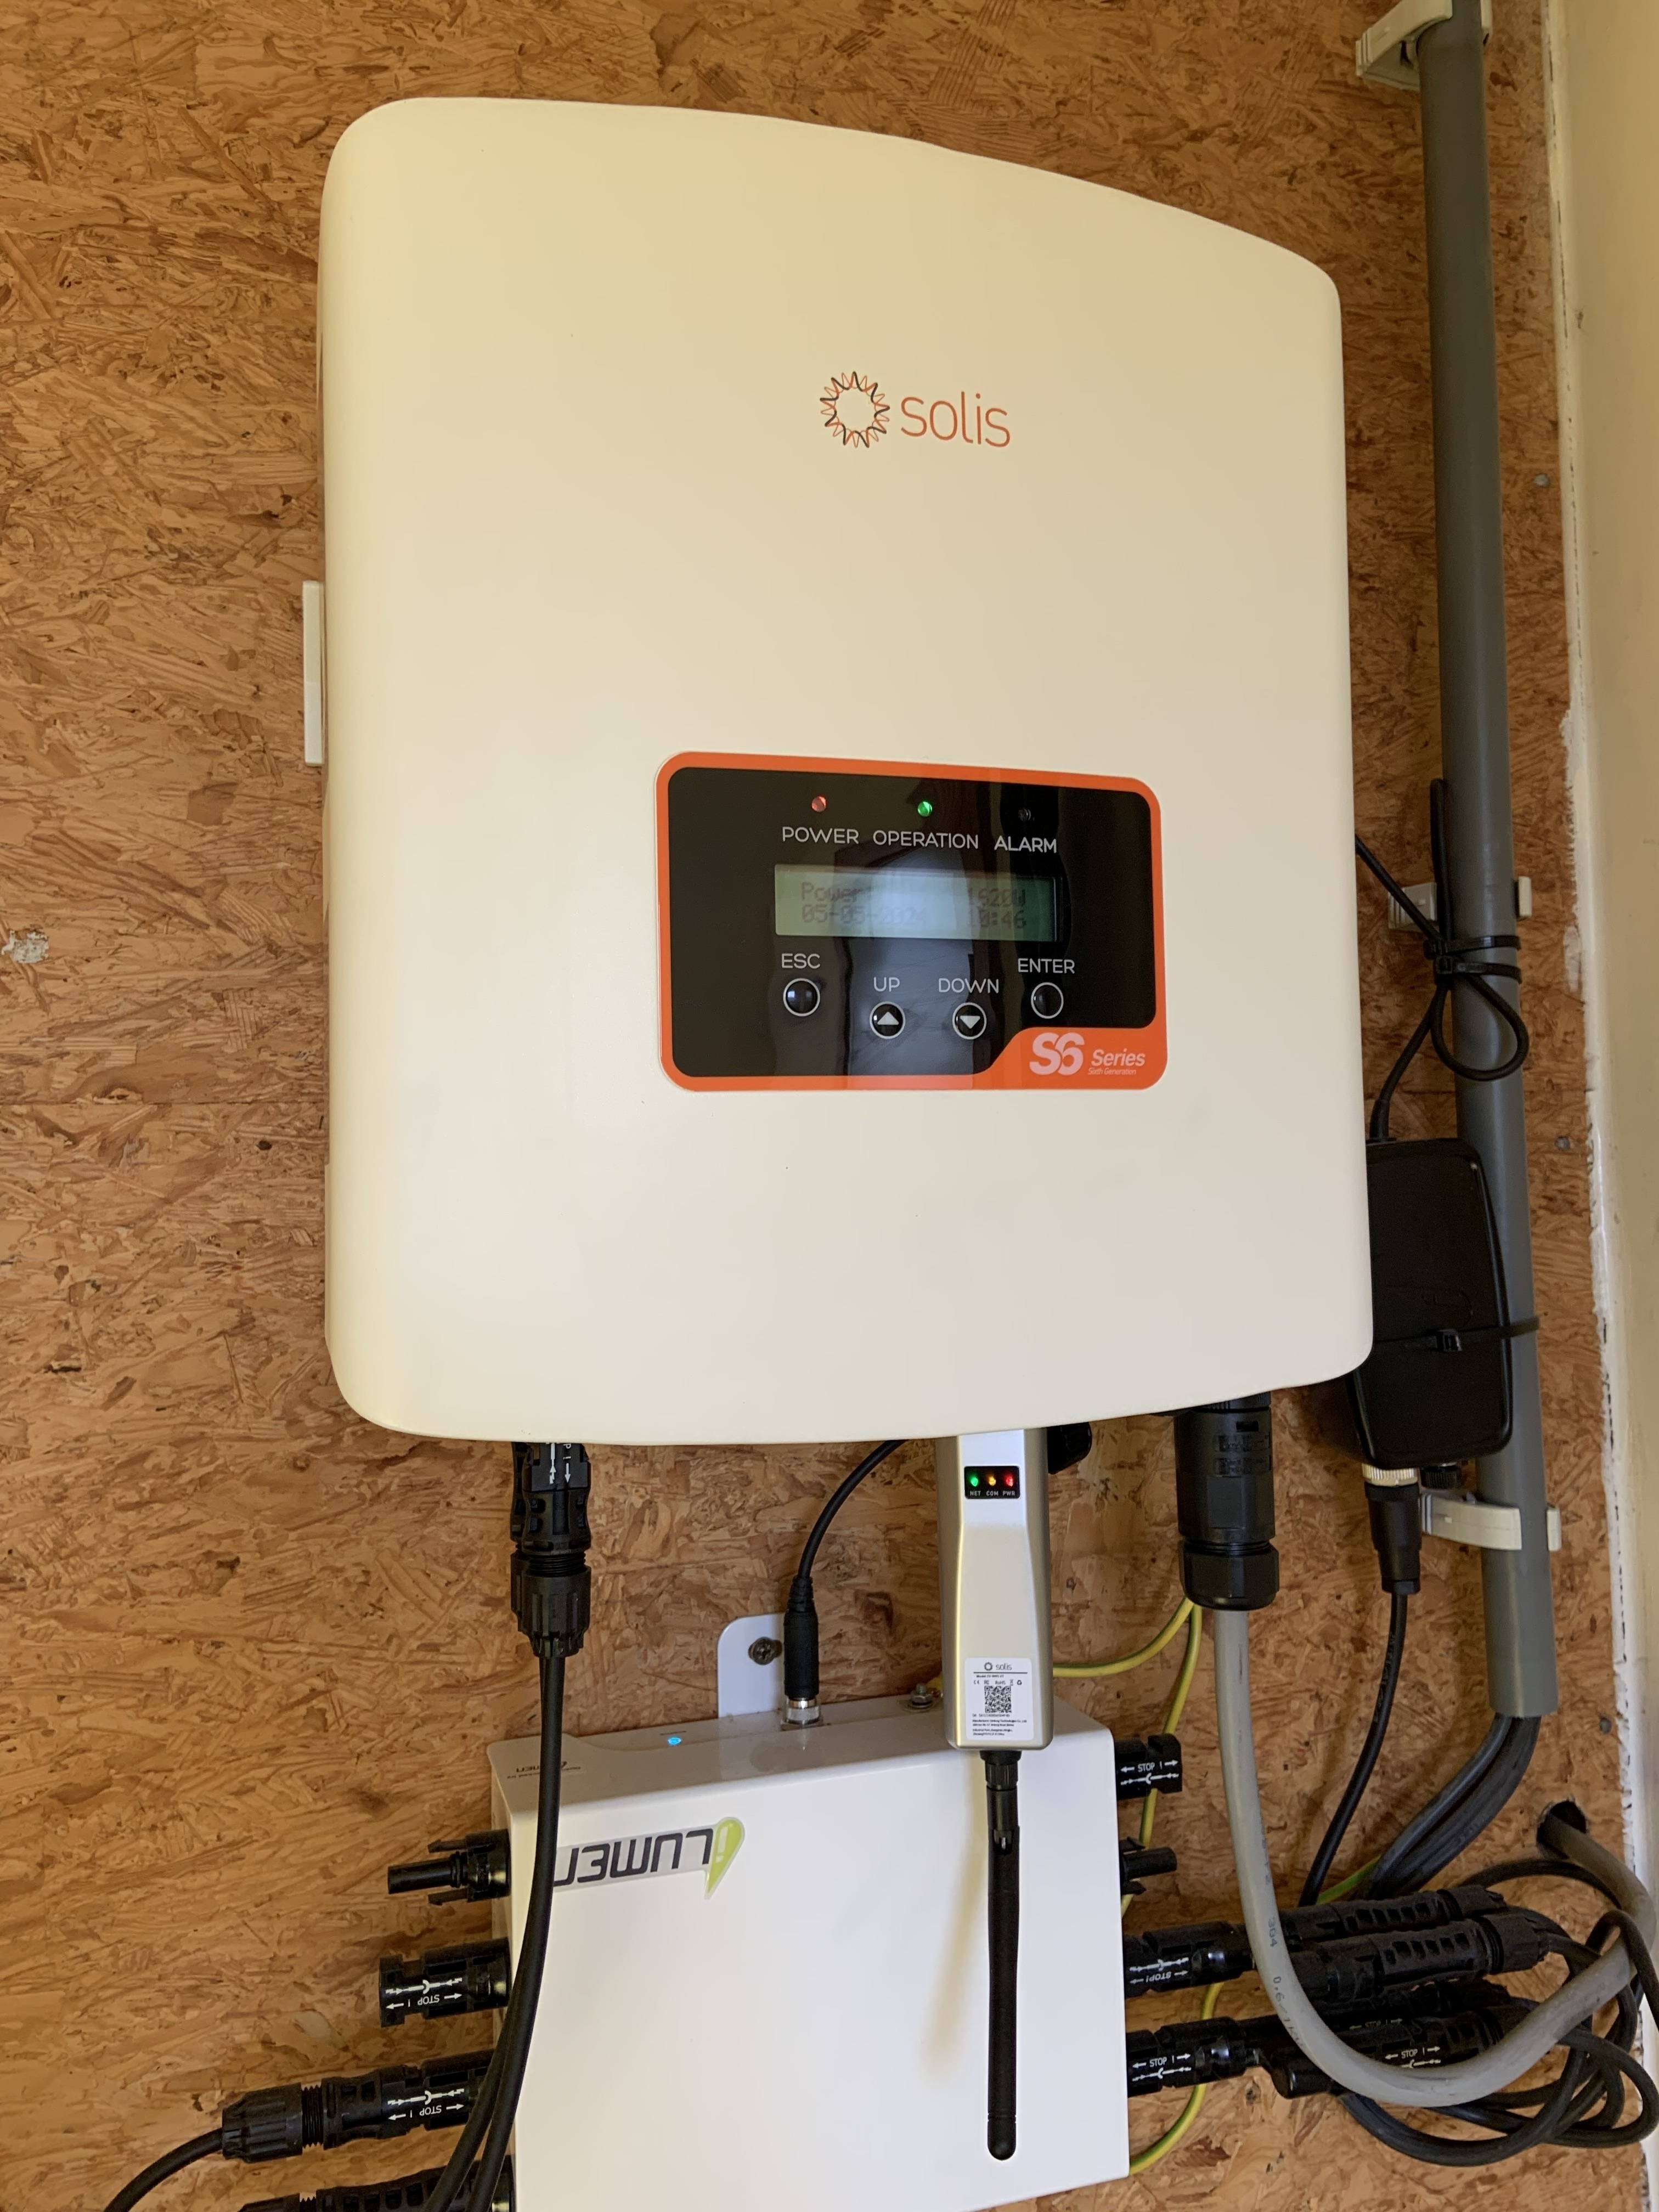
\includegraphics[width=7cm]{Omvormer} \hspace{0.5cm}
    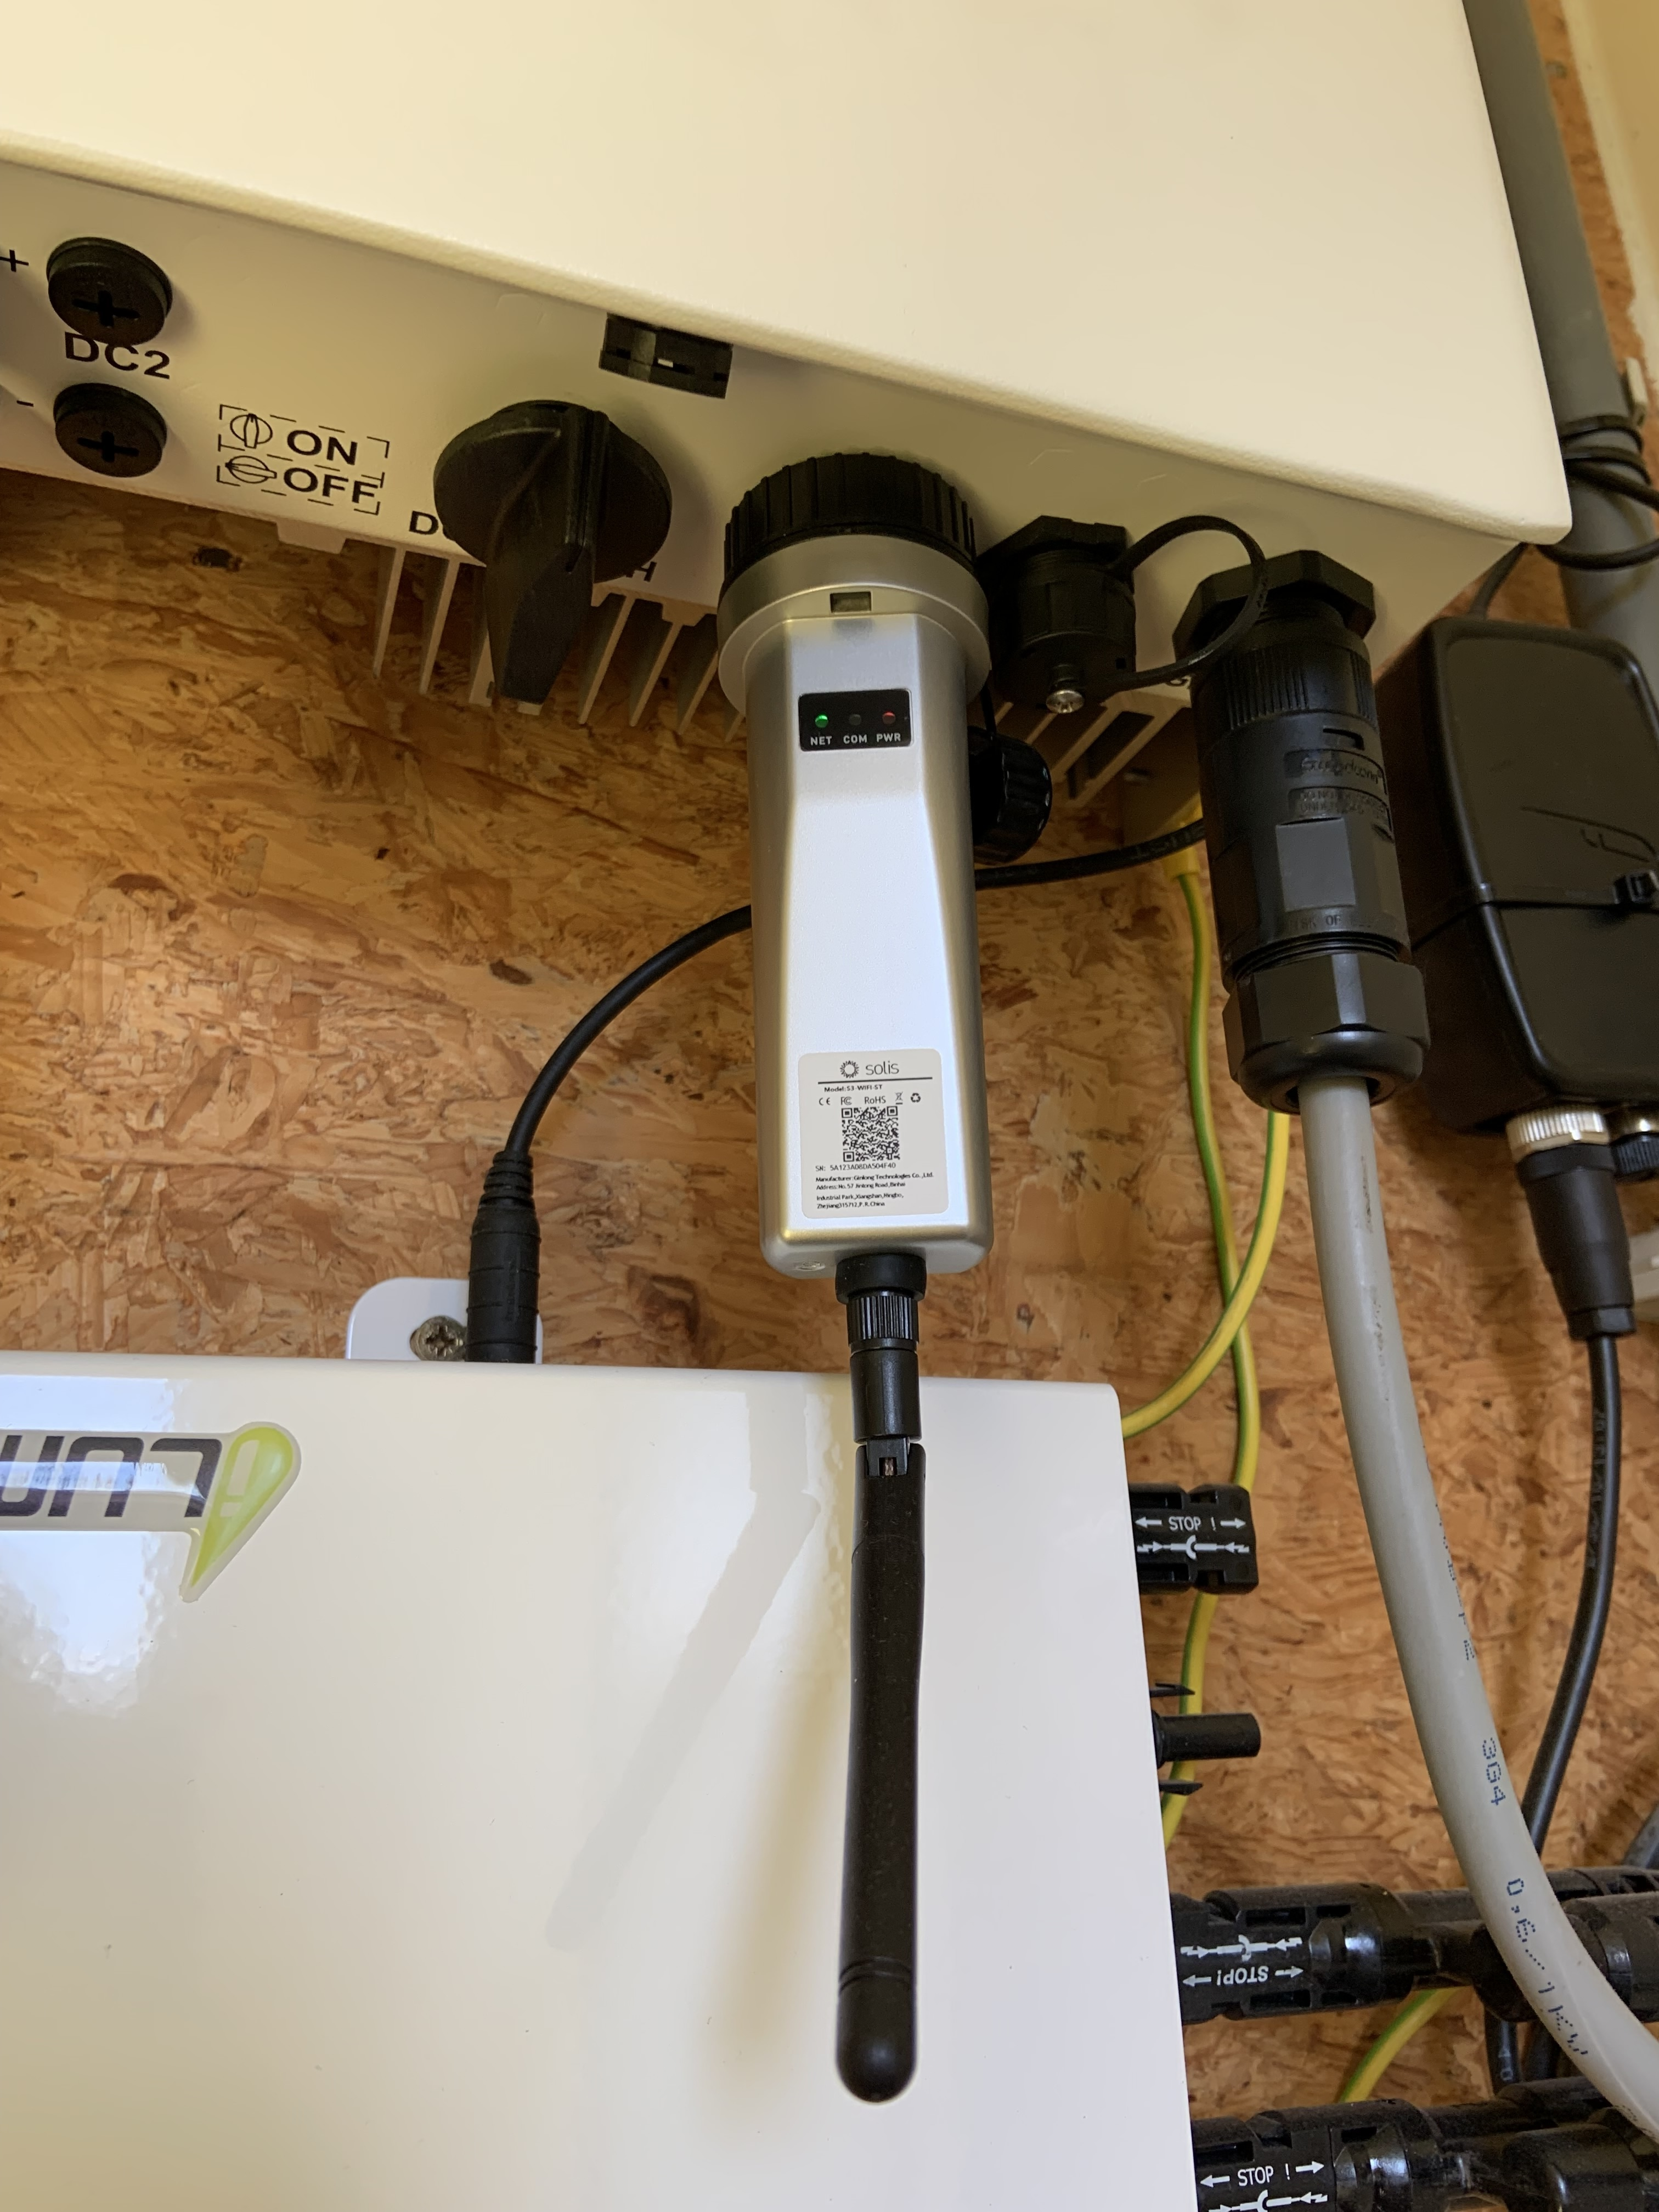
\includegraphics[width=7cm]{Wifi_Stick}
    \caption{Omvormer van de zonnepanelen met een wifi-stick.}
\end{figure}

Ook de data van de omvormer worden via het Python script weggeschreven naar een aparte InfluxDB databank en opgezet als een achtergrond service via de systeem manager voor Linux 'systemctl/systemd'. Zo blijft ook dit script automatisch uitgevoerd worden.

\subsection{\IfLanguageName{dutch}{Stroomproductie van zonnepanelen voorspellen met XGBoost}{Predicting power production PV system with XGBoost}}%
\label{sec:Stroomproductie van zonnepanelen voorspellen met XGBoost}

Het oorspronkelijke idee was om de stroomproductie van de zonnepanelen te gaan voorspellen op basis van de historische data van die stroomproductie. Voor dit onderzoek was er echter geen of slechts beperkte historische data voorhanden, omdat de metingen van de omvormer van de zonnepanelen pas gestart zijn bij het begin van het onderzoek. Na uitgebreid literatuuronderzoek werd beslist om de stroomproductie van de zonnepanelen te gaan voorspellen op basis van de hoeveelheid zonnestraling  \autocite{Sehrawat2023}, \autocite{Ledmaoui2023}, \autocite{Wang2022} en \autocite{Sansine2023}. Via de CAMS Radiation Service (CRS) van de Copernicus Atmosphere Monitoring Service (\href{https://atmosphere.copernicus.eu}{CAMS}) kan voldoende betrouwbare historische data met betrekking tot zonnestraling verkregen worden.

\subsubsection{Historische zonnestralingsdata verzamelen}

De zonnestralingsdata die via de CAMS Radiation Service (CRS) kan bekomen worden omvat tijdreeksen van globale, directe en diffuse instraling voor een tijdspanne van 1 februari 2004 tot en met 2 dagen geleden. De granulariteit van de data varieert van 1 maand tot 1 minuut en kan via een API-request opgevraagd worden. \\

Er bestaat een open-source Python library 'pvlib' \autocite{Jensen2023} die ontwikkeld werd om de opbrengst van zonnepanelen te simuleren. Deze library bevat ook tools om zonnestralingsdata op te vragen, waaronder de data van de CAMS Radiation Service (CRS). Omdat de reeds ontwikkelde scripts voor het uitlezen van de digitale elektriciteitsmeter en de omvormer van de zonnepanelen in Python geschreven zijn, worden ook de andere scripts in Python geschreven en kan de pvlib-library dus gebruikt worden. Om de zonnestralingsgegevens op te vragen moeten een aantal parameters worden meegegeven, waaronder de locatie (lengte- en breedtegraad), de start- en einddatum en de tijdsgranulariteit. Omdat van de gebruiker van de app niet kan verwacht worden dat hij of zij de geografische coördinaten van zijn of haar woning kent, wordt de Python library Geopy gebruikt om het ingevoerde adres van een gebruiker om te zetten in de correcte lengte- en breedgraad  coördinaten en deze vervolgens mee te geven in de API-call naar de CRS. \\

Voor dit onderzoek wordt de zonnestralingsdata voor een periode van iets meer dan 5 jaar opgevraagd, van 1 januari 2019 tot op heden om precies te zijn. Dat heden is evenwel de datum van 2 dagen eerder, aangezien het 2 dagen duurt vooraleer de CRS de waargenomen zonnestralingsdata verwerkt en opgeslagen heeft. Dit geeft voldoende data om via een machine learning algoritme de toekomstige hoeveelheid zonnestraling te gaan voorspellen. Voor de granulariteit werd geopteerd voor metingen om de 15 minuten. Zo zijn de metingen van de bekomen dataset voldoende gedetailleerd om accurate voorspellingen te kunnen maken, zonder dat de performantie in het gedrang komt. Bij metingen van 1 minuut blijkt de dataset te omvangrijk om er op een efficiënte en dus snelle manier berekeningen op uit te voeren.

\begin{figure}[h!]
    \centering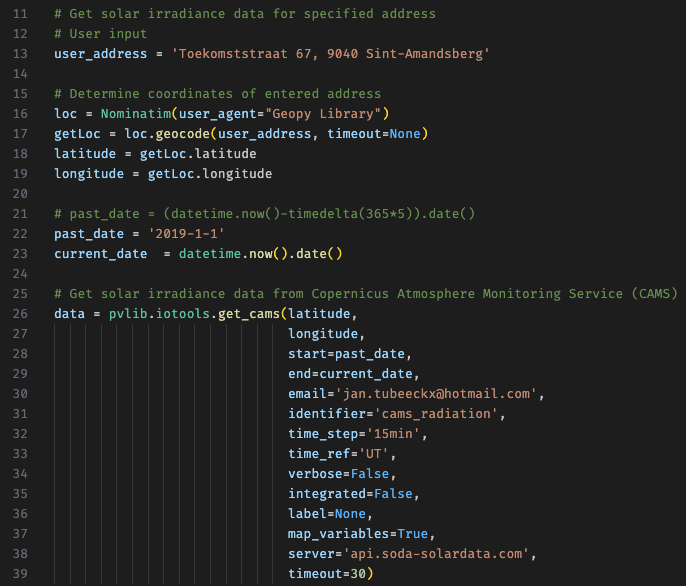
\includegraphics[scale=0.6]{Solar_Irradiance}
    \caption{\label{fig:Solar_Irradiance}Script voor het opvragen van de zonnestralingsdata.}
\end{figure} 

\newpage
\subsubsection{Weerdata}

Niet alleen de hoeveelheid zonnestraling is bepalend voor de stroomproductie van zonnepanelen, ook de weersomstandigheden oefenen een invloed uit. Vooral de omgevingstemperatuur, de relatieve luchtvochtigheid en de bewolkingsgraad zijn factoren die de stroomproductie van zonnepanelen kunnen vergroten of verkleinen \autocite{Sehrawat2023}. \\

Om de voorspelling van de toekomstige stroomproductie van de zonnepanelen accurater te maken, zal de zonnestralingsdata in de eerste plaats gecombineerd worden met historische weerdata voor dezelfde periode, van 1 januari 2019 tot op heden. Ook hiervoor werd gezocht naar een open-source API, waarmee de data via een Python script kan worden opgevraagd. Finaal is voor \href{https://dev.meteostat.net/}{Meteostat} gekozen. Deze API biedt een Pyhon library waarmee met slechts een enkele HTTP-request historische weerdata voor een bepaalde locatie kan worden opgevraagd. Meteostat verzamelt historische weer- en klimaatdata van weerstations en verschillende nationale meteorologische instituten van over de hele wereld. Omdat ook voor deze API-call de lengte- en breedtegraad van de gevraagde locatie moet worden ingegeven, wordt opnieuw gebruik gemaakt van de Python library Geopy waarmee een adres kan worden omgezet in de correcte lengte- en breedgraad coördinaten. \\

\begin{figure}[h!]
    \centering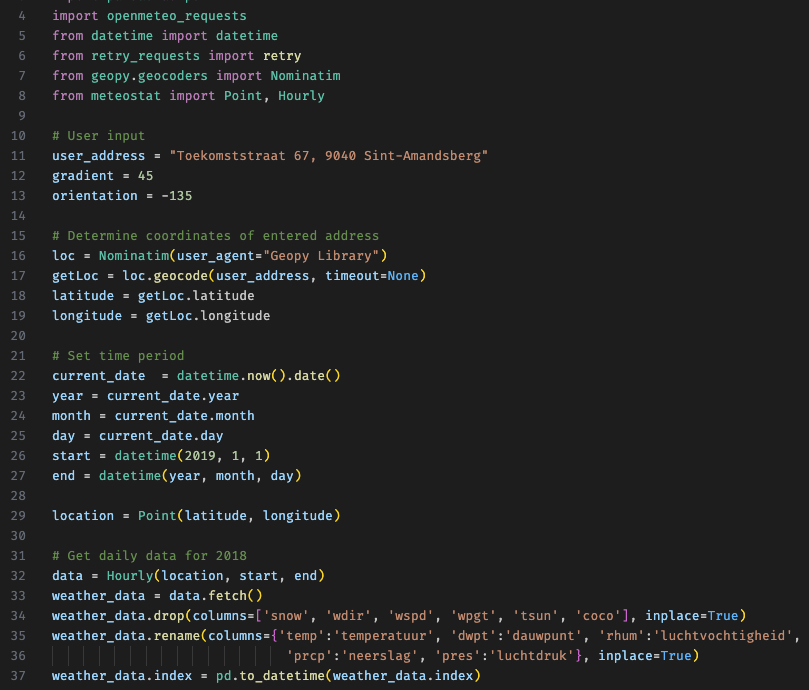
\includegraphics[scale=0.5]{Weerdata}
    \caption{\label{fig:Weerdata}Script voor het opvragen van de weerdata.}
\end{figure} 

Om de voorspelling van de stroomproductie van de zonnepanelen nog beter te maken, zal de bekomen voorspelling gecombineerd worden met de weersvoorspellingen voor de voorspelde periode. Aangezien Meteostat enkel historische data aanbiedt, moest een andere open-source weer-API gevonden worden. \href{https://open-meteo.com/}{Open-Meteo API} werkt ook samen met verschillende nationale meteorologische diensten waardoor het betrouwbare weersvoorspellingen aanbiedt. De aangeboden API-request is makkelijk in te stellen, zodat enkel de benodigde weerdata kan worden opgevraagd. Zo kan de data snel opgevraagd worden. Voor dit onderzoek worden enkel de voorspellingen van de omgevingstemperatuur, de relatieve luchtvochtigheid en de bewolkingsgraad opgehaald.

\subsubsection{Voorspelling met XGBoost}

Door het toenemend belang van hernieuwbare energie is er al heel wat onderzoek verricht naar het voorspellen van de elektriciteitsproductie van PV-systemen door toepassing van machine learning. Uit de meest recente onderzoeken blijkt dat Extreem Gradient Boosting (XGBoost) andere machine learning algoritmes overtreft bij het voorspellen van historische zonnestraling \autocite{Khasawneh2024}, \autocite{Tercha2024},  \autocite{Ledmaoui2023}, \autocite{Wang2022} en \autocite{BarreraAnimas2022}. Om die reden wordt voor dit onderzoek gebruik gemaakt van XGBoost om de toekomstige zonnestraling en vervolgens de stroomproductie van zonnepanelen te voorspellen. 

\subparagraph{Data cleaning en correlaties}
De dataset die als invoer voor het XGBoost algoritme gebruikt werd, is dus een combinatie van historische zonnestralingsdata en weerdata. Deze datset werd eerst gezuiverd van anomalieën door alle negatieve en ontbrekende waarden te verwijderen, anders zouden deze fouten de voorspelde waarden kunnen vertekenen. Na het opschonen van de data werden bestaande correlaties onderzocht. Hiervoor werd de Python library 'Seaborn' gebruikt, waarmee een heatmap van de correlaties tussen de verschillende kenmerken van de dataset kon worden opgemaakt. Daaruit blijkt inderdaad dat vooral de omgevingstemperatuur (positief) en luchtvochtigheid (negatief) het sterkst correleren met de globale horizontale instraling van de zon (GHI). 

\begin{figure}[h!]
    \centering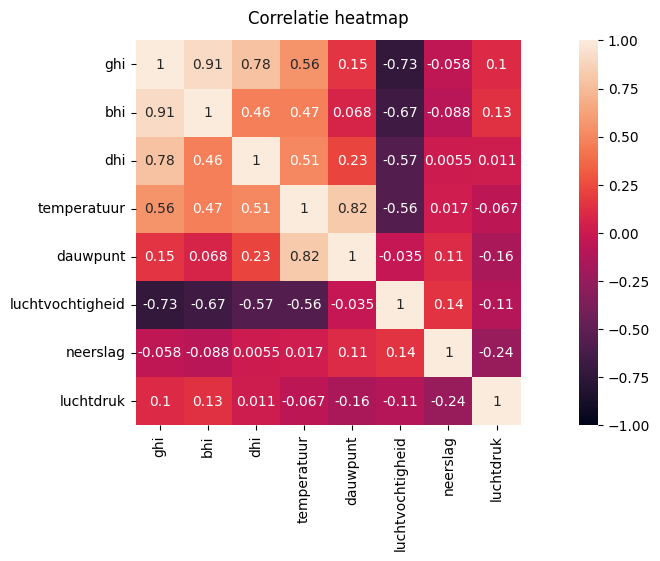
\includegraphics[scale=0.7]{correlatie}
    \caption{\label{fig:correlatie}Heatmap van correlaties tussen de verschillende kenmerken van de dataset.}
\end{figure} 

\newpage
\subparagraph{Toevoeging van features}
De historische zonnestralingsdata die gebruikt wordt, kan beschouwd worden als tijdreeksen (time-series) vermits de data geordend is volgens een tijdsindex. Om de analyse van deze tijdreeksen te verbeteren en patronen in de zonnestralingsdata vast te stellen, worden extra 'Features' of tijdgerelateerde kenmerken  toegevoegd aan de gebruikte dataset. Deze kenmerken worden afgeleid van de index van de dataset die uit het tijdstip van de gemeten waarde bestaat (zie figuur 4.6). Deze verrijking zorgt voor een beter begrip van de tijdsgebonden aspecten van de gegevens en het later toegepaste XGBoost model bij het herkennen van patronen en seizoensgebondenheid.  

\begin{figure}[h!]
    \centering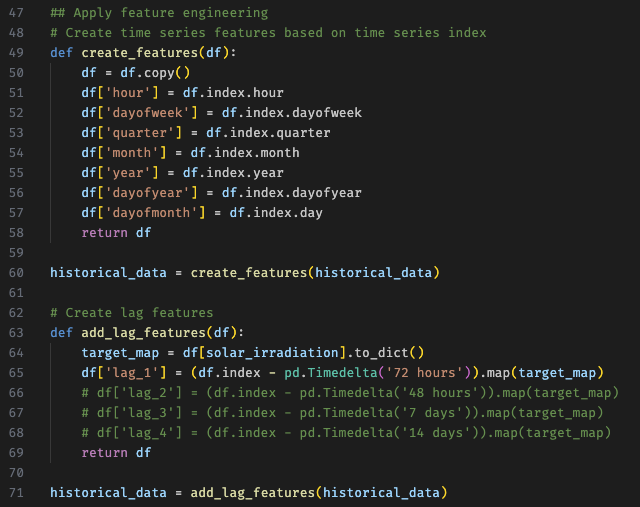
\includegraphics[scale=0.6]{Features_Lags}
    \caption{\label{fig:Features_Lags}Screenshot van de Python code voor het aanmaken van features en lags.}
\end{figure} 

\subparagraph{Toevoeging van lag features}
Om het XGBoost algoritme nog beter in staat te stellen om tijdsgebonden afhankelijkheden en verbanden te herkennen, worden zogenaamde 'lag features' of vertragingskenmerken aan de dataset toegevoegd. Hiermee wordt het algoritme opgedragen om de zonnestralingswaarden van een bepaald aantal dagen in het verleden op te nemen als nieuwe features. De toevoeging van lag features zorgt opnieuw voor een verrijking van de dataset en voorziet het model van historische informatie om zonnestralingspatronen beter te begrijpen en te voorspellen, wat uiteindelijk bijdraagt aan de nauwkeurigheid en effectiviteit van het XGBoost model \autocite{Nabatchian2024}.

\subparagraph{XGBoost model trainen en testen}
Omdat het XGBoost model heel wat parameters bevat die kunnen aangepast worden, werden verschillende versies ontwikkeld en getest. Om elke versie te kunnen beoordelen werd de gebruikte dataset opgesplitst in een trainingset en een testset. Daarbij werd het algoritme getraind op de trainigset en beoordeeld op testset. Omdat de data uit tijdreeksen bestaat, werd voor het opsplitsen van de dataset geopteerd voor de 'TimeSeriesSplit' functie van de Scikit-learn library. Deze functie is speciaal ontworpen voor de opsplitsing van tijdreeksgegevens en zorgt ervoor dat de chronologische volgorde van de gegevens behouden blijft tijdens het opsplitsingsproces. Dit zorgt voor een grotere nauwkeurigheid van de beoordeling van de voorspellingscapaciteit van het model.

\begin{figure}[h!]
    \centering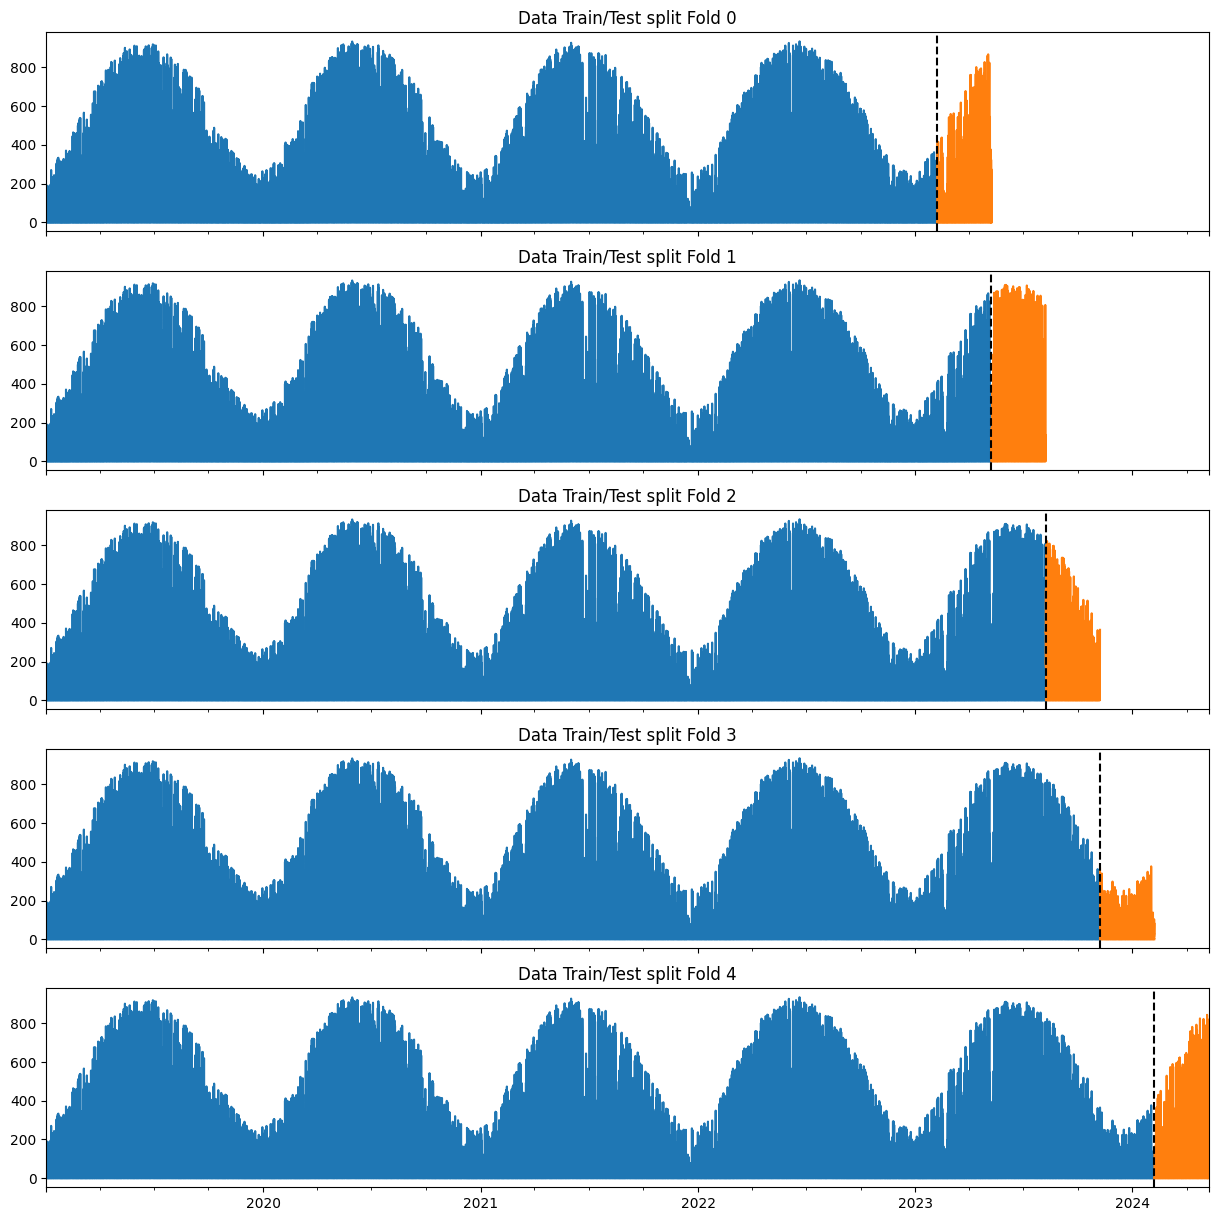
\includegraphics[scale=0.45]{TimeSeriesSplit}
    \caption{\label{fig:TimeSeriesSplit}Grafische voorstelling van de TimeSerieSplit functie.}
\end{figure} 

Om de geteste modellen te beoordelen werd telkens de mean absolute error (MAE), mean squared error (MSE) en root mean squared error (RMSE) over de verschillende opsplitsingen heen berekend. Het uiteindelijk gekozen model behaalde volgende scores: MAE score van 0.5519, MSE score van 1.5816 en RMSE score van 1.2576.

\subparagraph{Voorspelling van de zonnestraling}

Om de toekomstige zonnestaling te voorspellen werd het geselecteerde algoritme getraind op de volledige dataset met alle historische data, zonder een opsplitsing te maken tussen een training- en testset. De bekomen voorspelling van de zonnestraling werd vervolgens gecombineerd met de voorspelling van de omgevingstemperatuur en de relatieve luchtvochtigheid die via de Open-Meteo API voor dezelfde periode werd opgehaald. 

\begin{figure}[h!]
    \centering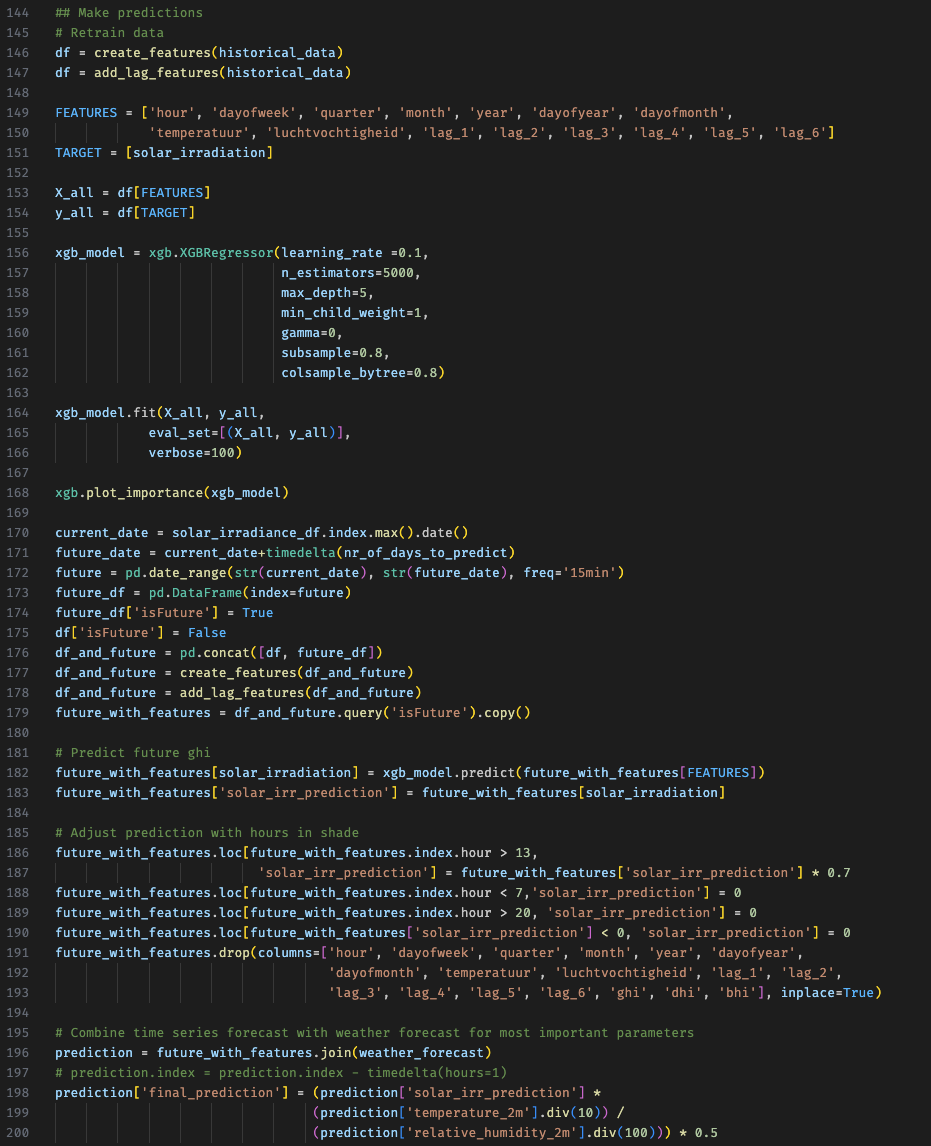
\includegraphics[scale=0.42]{Prediction}
    \caption{\label{fig:Prediction}Screenshot van de Python code voor de voorspelling van de zonnestraling van de volgende dag.}
\end{figure} 

\subparagraph{Omzetting voorspelde zonnestraling naar opgewekte stroom}

Op basis van de gecombineerde voorspelling van de zonnestraling (GHI) kan vervolgens de toekomstige stroomproductie van de zonnepanelen berekend worden. Daarbij geldt dat het opgewekte vermogen van zonnepanelen lineair toeneemt naarmate de zonnestraling (GHI) toeneemt, en lineair afneemt naarmate de omgevingstemperatuur toeneemt. Het opgewekte vermogen van de zonnepanelen kan dan berekend worden door de formule

\begin{figure}[h!]
    \centering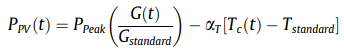
\includegraphics[scale=0.7]{PVPower_Formula}
\end{figure} 

waarbij 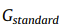
\includegraphics[height=1.7em]{Gstandard} en 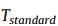
\includegraphics[height=1.7em]{Tstandard} verwijzen naar de standaard testcondities die fabrikanten van zonnepanelen hanteren \autocite{Kazem2017}. Deze standaard test condities zijn 1000 W/m² zonnestraling en een omgevingstemperatuur van 25\textdegree C. \\ 

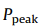
\includegraphics[height=1.7em]{PPeak} verwijst naar het piekvermogen van de zonnepanelen. Dit piekvermogen(Wp) wordt onder bovenstaande omstandigheden door de fabrikant bepaald. \\

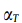
\includegraphics[height=1.5em]{Temp_Coeff} verwijst naar de temperatuur-coëfficiënt. Deze waarde geeft aan wat de invloed is van de temperatuur van de zonnepanelen op het rendement van de zonnepanelen. De meeste zonnepanelen hebben een temperatuurcoëfficiënt van ongeveer -0,35 \% per graad Celsius. Dat betekent dat het vermogen ongeveer met 1\% afneemt bij een stijging van 3 graden Celsius. \\

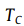
\includegraphics[height=1.5em]{Cell_Temp} tenslotte verwijst naar de zonneceltemperatuur en word berekend via volgende fomule:

\begin{figure}[h!]
    \centering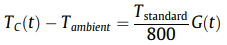
\includegraphics[scale=0.7]{CellTemp_Formula}
\end{figure} 

De PV-installatie die voor dit onderzoek gebruikt werd, bestaat uit 10 zonnepanelen die elk een piekvermogen van 215 Watt hebben. Dit geeft een totaal piekvermogen van 2.150 Watt. Zonnepanelen behalen echter nooit hun volledige piekvermogen omdat de weers- en omgevingsfactoren anders zijn dan de bovenvermelde standaard testcondities die door de fabrikanten gebruikt worden. In België moet rekening gehouden worden met een omgevingsfactor van 0,85. Dit betekent dat het werkelijke piekvermogen van de zonnepanelen slechts 1.827,50 Watt is (2.150 Watt x 0,85). De zonnepanelen die in dit onderzoek gebruikt werden, zijn echter al 25 jaar oud en uit de metingen gedurende anderhalve maand blijkt dat zij nog maar 76\% van hun piekvermogen halen, zijnde 1.634 Watt. \\

\newpage
\subsection{\IfLanguageName{dutch}{Weergave uitgelezen data en voorspelling met een iOS app}{Display of data and prediction with an iOS app}}%
\label{sec:Weergave uitgelezen data en voorspelling met een iOS app}

Omdat een smartphone makkelijker en vaker consulteerbaar is, werd in dit onderzoek geopteerd voor de ontwikkeling van een mobiele app om de elektriciteitscon- sumptie- en productie weer te geven en op te volgen. De app is ontwikkeld voor iOS omdat dit het testen achteraf vergemakkelijkt. De iOS-app werd gebouwd in de geïntegreerde ontwikkelomgeving (IDE) XCode met SwiftUI en UIKit. Voor documentatie en tutorials werd gebruik gemaakt van het \href{https://developer.apple.com/}{Apple developer platform}. \\

Om de uitgelezen data van de digitale elektriciteitsmeter en de omvormer van de zonnepanelen beschikbaar te maken voor de app, werd eerst een webserver geïnstalleerd op de Raspberry Pi. Daarvoor werd Flask gebruikt. Dit is een open-source Python web framework, waarmee op een eenvoudige manier webapplicaties gebouwd kunnen worden. Het is een micro-framework wat betekent dat het weinig tot niet afhankelijk is van externe libraries en zeer licht is. Omdat de backend voor de ontwikkelde app eerder beperkt is en de webserver op een minicomputer moet draaien, is Flask de meest voor de hand liggende keuze \autocite{Shokrzad2023}. Met de toevoeging van één enkel bijkomend Python bestand konden alle nodige REST-calls opgezet worden. 

\subsubsection{Elektriciteitsconsumptie en -productie}
De ontwikkelde app geeft de gebruiker vooreerst een overzicht van zijn of haar elektriciteitsverbruik- en productie. 

\begin{figure}[h!]
    \centering
    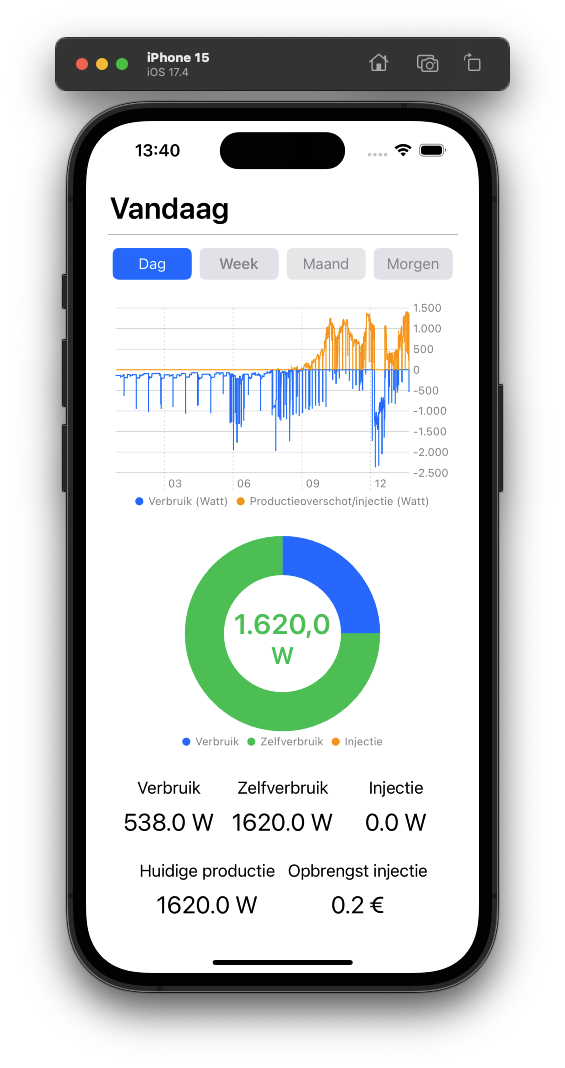
\includegraphics[width=5cm]{Iphone_dag_cons} \hspace{0.1cm}
    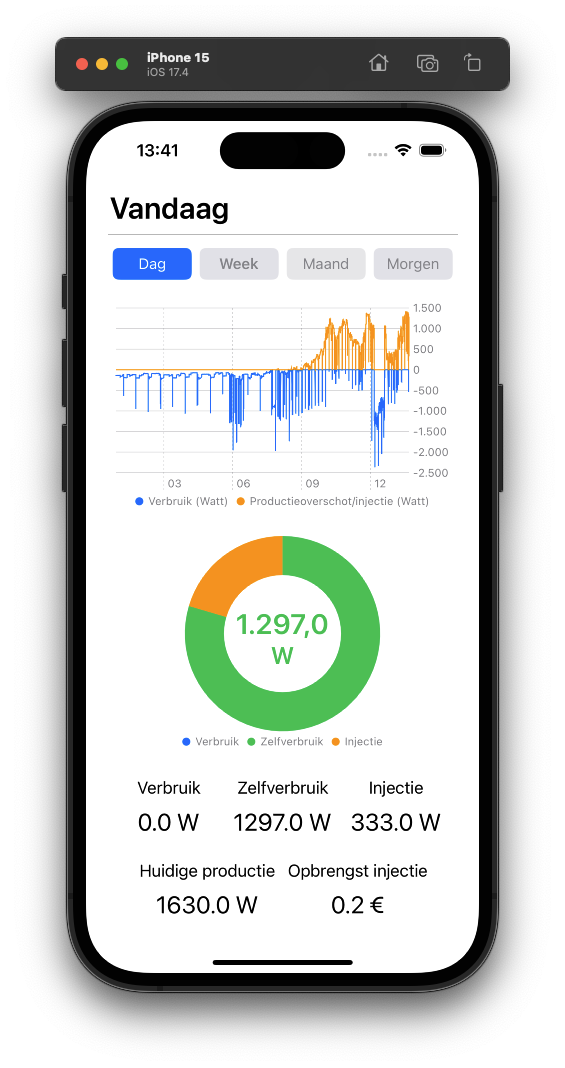
\includegraphics[width=5cm]{Iphone_dag_self} \hspace{0.1cm}
    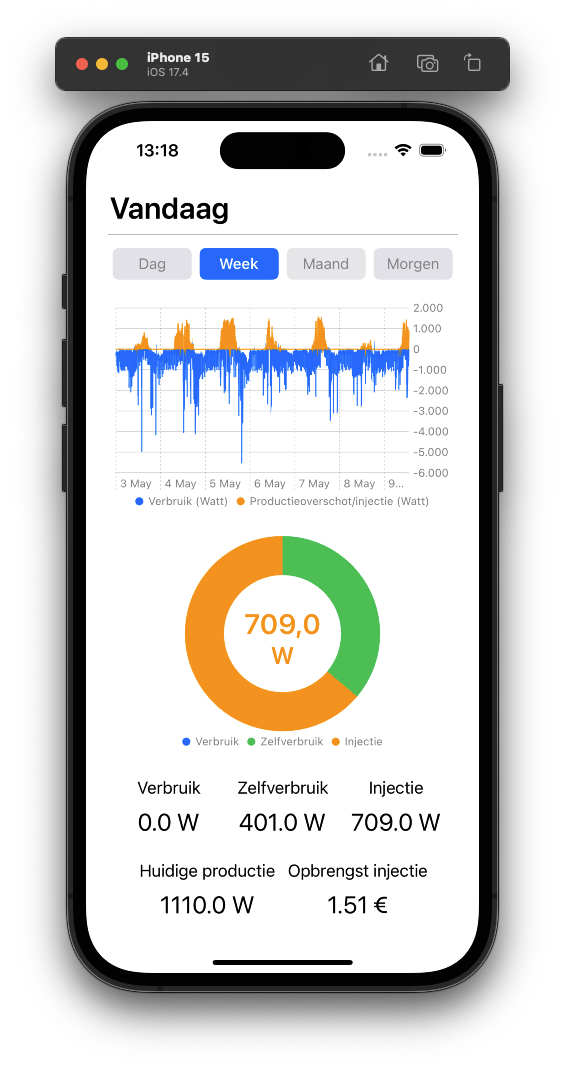
\includegraphics[width=5cm]{Iphone_week}
    \caption{Overzicht elektricteitsverbruik en -productie per dag en per week.}
\end{figure}

Op een eerste grafiek worden per periode (dag, week, maand) het verbruik en productieoverschot getoond. Dit productieoverschot is de zelf geproduceerde stroom die niet verbruikt wordt en dus in het distributienetwerk geïnjecteerd wordt. Voor deze injectie ontvangt de gebruiker een beperkte vergoeding van zijn of haar stroomleverancier. Het doel van het onderzoek van deze bachelorproef is niet enkel om het elektriciteitsverbruik beter te gaan spreiden, maar ook om ervoor te zorgen dat de zelf geproduceerde stroom van de zonnepanelen effectief zelf verbruikt wordt. Het bedrag van de vergoeding voor de geïnjecteerde stroom is immers dermate laag dat het financieel voordeliger is om de zelfgeproduceerde elektriciteit zelf te gebruiken, dan deze stroom te verkopen. Om die reden wordt het bedrag van de opbrengst van de geïnjecteerde stroom gedurende de geslecteerd periode aan de gebruiker getoond. Zo heeft deze een besef van het voordeel dat zelfverbruik hem of haar oplevert. \\

Op een tweede grafiek worden de huidige consumptie- en productiegegevens getoond. Zo ziet de gebruiker duidelijk hoeveel elektriciteit hij of zij van het net afneemt en dus betaalt, hoeveel van de zelf opgewekte stroom hij of zij effectief zelf gebruik en hoeveel van de zelfgeproduceerde stroom geïnjecteerd en dus verkocht wordt. Daarbij wordt in het midden van de grafiek de grootste van deze drie waarden getoond, zodat de gebruiker meteen ziet wat er overheerst: zijn of haar verbruik, zelfconsumptie of injectie. \\

Tot slot worden onder de beide grafieken de consumptie- en productiedetails als waarden getoond. Zo ziet de gebruiker ook de totale hoeveelheid elektriciteit die door de zonnepanelen wordt opgewekt.

\subsubsection{Voorspelling stroomproductie}

Via de app kan ook de voorspelde stroomproductie van de volgende dag geraadpleegd worden. Deze voorspelling is het resultaat van het Python script waarmee het XGBoost algoritme en de voorspelling van de stroomproductie geïmplementeerd werd. Dit script wordt automatisch om het uur uitgevoerd, zodat steeds een recente voorspelling kan getoond worden. De gemaakte voorspelling wijzigt immers doorheen de dag. Het is op basis van deze voorspelling dat de app automatisch sanitaire of andere apparaten zal gaan inschakelen wanneer er voldoende stroomproductie voorspeld wordt. 

\begin{figure}[h!]
    \centering
    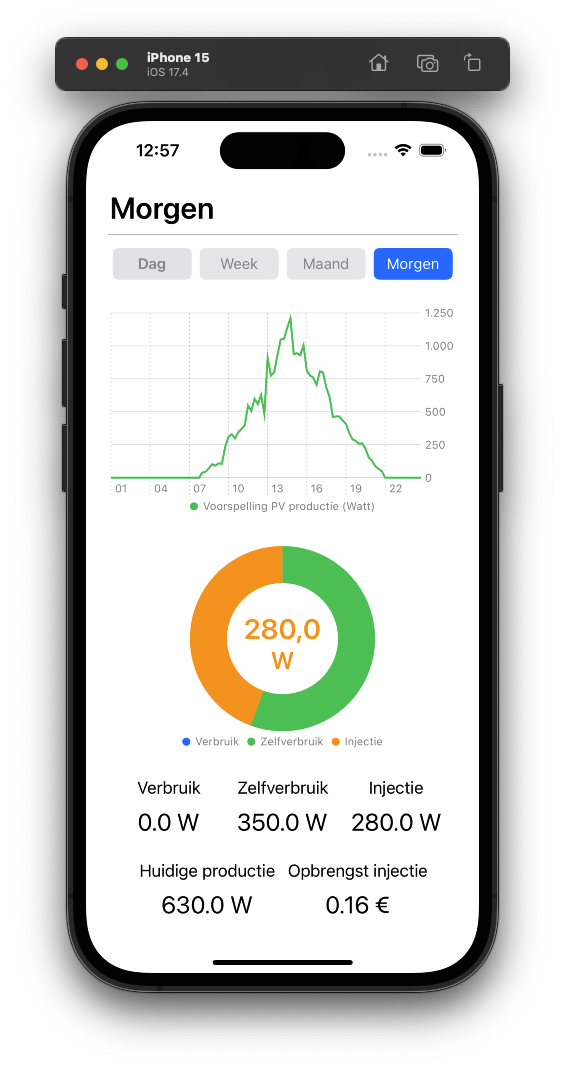
\includegraphics[width=5cm]{Iphone_prediction} \hspace{0.5cm}
    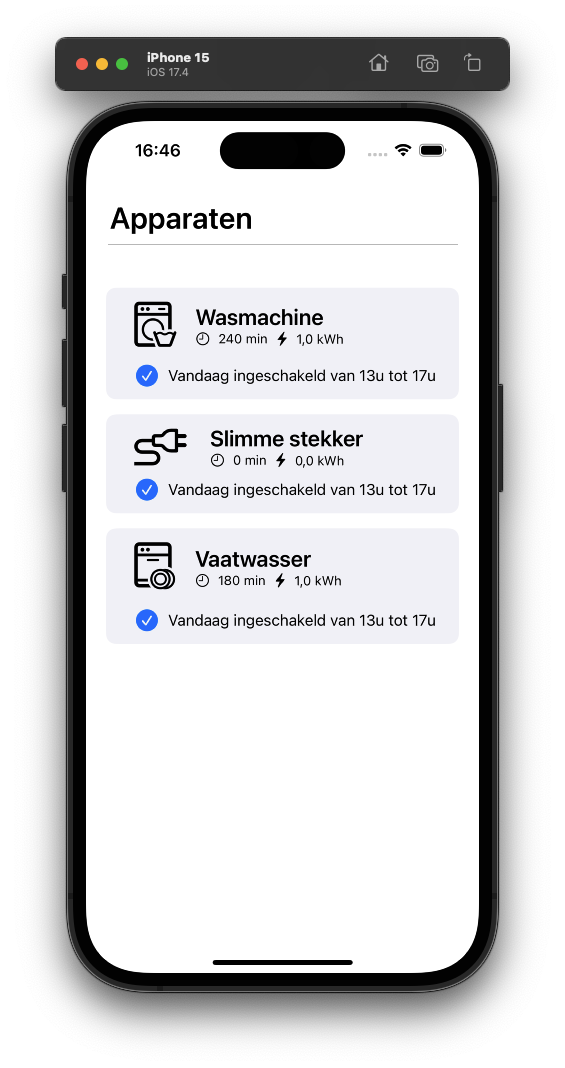
\includegraphics[width=5cm]{Device_List}
    \caption{Voorspelling van de stroomproductie en overzicht van de ingeschakelde apparaten.}
\end{figure}

\newpage
\subsection{\IfLanguageName{dutch}{Aansturing slimme apparaten op basis van de voorspelde stroomproductie}{Predicting power production PV system with XGBoost}}%
\label{sec:Aansturing slimme stekkers aansturen op basis van de voorspelde stroomproductie}

De gebruiker zal via de app toestellen kunnen toevoegen die automatisch ingeschakeld mogen en kunnen worden wanneer er voldoende stroomproductie voorspeld wordt. De app zal de gebruiker adviseren over welke apparaten het best kunnen worden toegevoegd omdat ze het meeste verbruiken. Denk daarbij in de eerste plaats aan een warmtepomp of laadpaal indien deze aanwezig zijn, maar ook aan de wasmachine en de vaatwasser. De app zal zelf het verbruik en de inschakelduur van het apparaat gaan bepalen. Indien bijvoorbeeld een wasmachine wordt toegevoegd, dan zal de app het verbruik instellen op 1 kWh en ervan uitgaan dat een wasprogramma gemiddeld 3 uur duurt. De gebruiker zal evenwel de mogelijkheid hebben om dit verbruik en de inschakeltijd zelf te gaan instellen, net zoals hij de mogelijkheid heeft om de inschakeling van een apparaat handmatig te verhinderen.\\

Wanneer uit de voorspelling van de stroomproductie blijkt dat er voldoende elektricteit zal worden opgewekt de volgende dag, zal de app de toestellen die de gebruiker heeft toegevoegd gaan inplannen voor de volgende dag. Dit was althans de theorie, want bij de selectie van de toestellen voor dit onderzoek bleek dat de toestellen van het huis dat als testopstelling diende nog niet 'slim' waren. Een probleem dat zich helaas zal voordoen bij heel wat gezinnen. Om dit op te vangen werd gebruik gemaakt van slimme stekkers. Dit zijn stekkers die via wifi kunnen in- en uitgeschakeld worden. Zij worden tussen het klassieke stopcontact en de stekker van het toestel geplaatst, waardoor een toestel op een eenvoudige manier slim kan gemaakt worden \autocite{Jong2020}. Maar ook daarbij stelde zich een probleem. Een slimme stekker kan enkel stroom doorlaten of tegenhouden. Dit vereist dat een toestel reeds kan ingeschakeld worden indien het geen stroom krijgt en dat het dus zonder tussenkomst van een gebruiker kan opstaren van zodra de slimme stekker stroom doorlaat. De sanitaire toestellen van de testopstelling voor dit onderzoek, konden pas worden aangezet nadat ze stroom kregen én op een elektronische startknop geduwd werd. \\

Om de werking van de app in combinatie met slimme stekkers toch te testen, werd een slimme stekker verbonden met een staande lamp. Op die manier kan duidelijk worden waargenomen wanneer de slimme stekker was ingeschakeld. De aansturing van de slimme stekker gebeurt via een Python script dat als een service op de Raspberry Pi minicomputer uitgevoerd wordt. In dit script wordt de slimme stekker bestuurd met behulp van een Python library PyP100 die speciaal ontwikkeld werd voor het gebruikte merk van stekker. Via deze library kan verbinding gemaakt worden met de slimme stekker door het IP-adres en de inloggegevens mee te geven. 

\begin{figure}[h!]
    \centering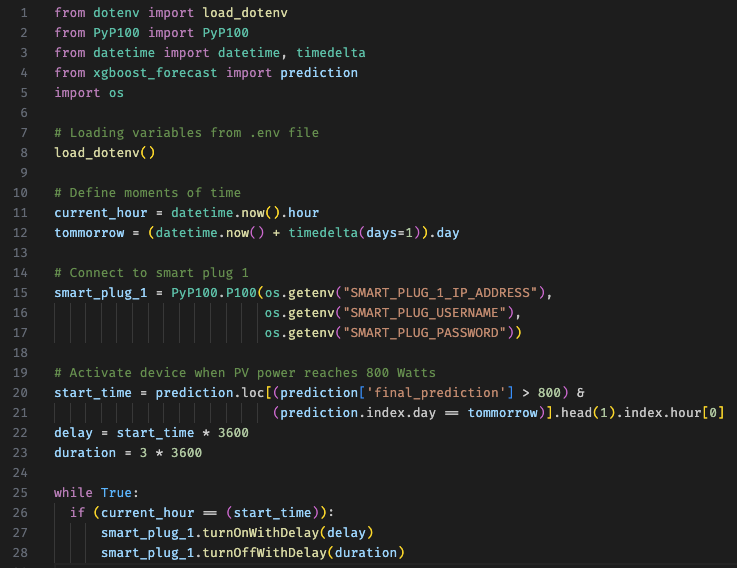
\includegraphics[scale=0.53]{SmartPlug_Script}
    \caption{\label{fig:SmartPlug_Script}Screenshot van de Python code om de slimme stekker aan te sturen op basis van de voorspelde stroomproductie.}
\end{figure} 

Het script is zo geprogrammeerd dat het elke dag om 23u zal uitgevoerd worden. Het vraagt daarbij eerst de voorspelling van de stroomproductie van de volgende dag op. Vervolgens zal de slimme stekker geprogrammeerd worden om de volgende dag in te schakelen van zodra de voorspelde waarde van de opgewekte stroom 800 Watt of meer bedraagt. Op de dag zelf kan de gebruiker in de app een overzicht kunnen raadplegen van de ingeschakelde apparaten met hun tijdschema.